\begin{figure*}[ht!]
\begin{center}% note that \centering uses less vspace...
\resizebox{2\columnwidth}{!}{%
\begin{tabular}{lllll}


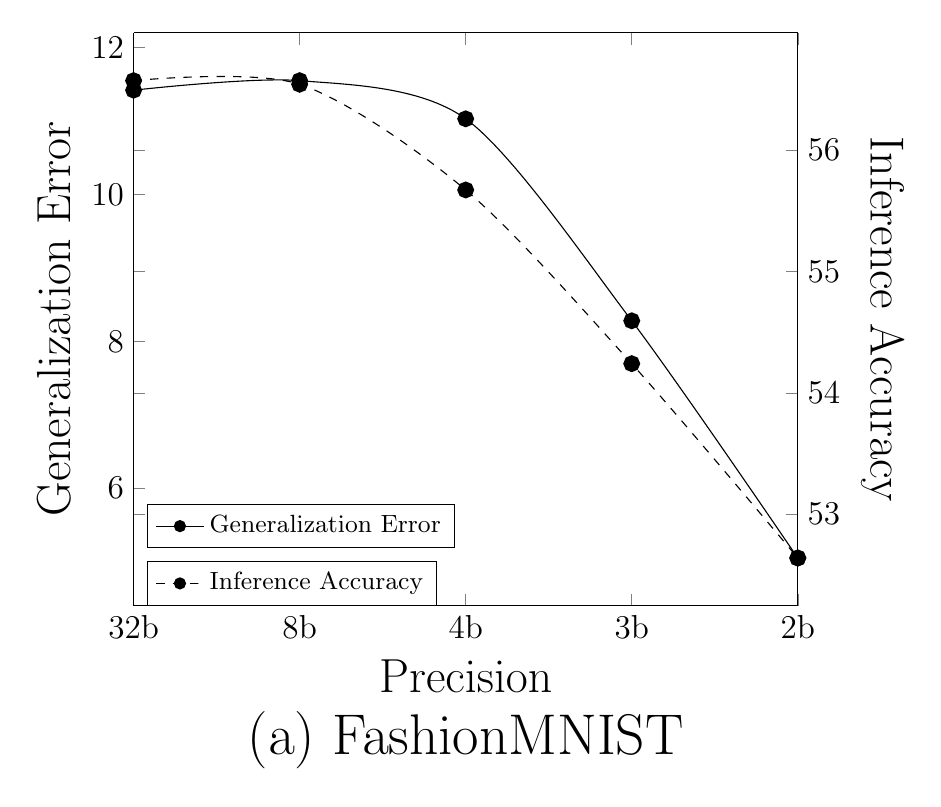
\begin{tikzpicture}
% let both axes use the same layers
\pgfplotsset{set layers}
%
\begin{axis}[
title={(a) FashionMNIST},
title style={at={(0.5,0)},anchor=north,yshift=-40, font=\huge},
scale only axis,
line width=2.0pt,
mark size=2.0pt,
xmin=0,xmax=4,
ylabel={Generalization Error},
axis y line*=left,
xlabel={Precision},
xtick={0,1,2,3,4},
xlabel style={font=\LARGE},
ylabel style = {font=\LARGE},
xticklabel style = {font=\large},
yticklabel style = {font=\large},
xticklabels={32b, 8b, 4b, 3b, 2b},
legend style={at={(0.02,0.1)},anchor=south west, font=\small}
]
\addplot[
    color=black,
    solid,
    mark=*,
    mark options={solid},
    smooth
    ]
    coordinates {
    (0,11.42)(1,11.55)(2,11.03)(3,8.28)(4,5.05)
      };
      \addlegendimage{color=black,solid,mark=*, mark options={solid}}
      \addlegendentry{Generalization Error}
\end{axis}

\begin{axis}[
scale only axis,
line width=2.0pt,
mark size=2.0pt,
xmin=0,xmax=4,
ylabel near ticks, yticklabel pos=right,
ylabel={Inference Accuracy},
ylabel style = {rotate=180, font=\LARGE},
yticklabel style = {font=\large},
axis x line=none,
legend style={at={(0.02,0)},anchor=south west, font=\small}
]
\addplot[
    color=black,
    dashed,
    mark=*,
    mark options={solid},
    smooth
    ]
    coordinates {
    (0,56.57)(1,56.54)(2,55.67)(3,54.24)(4,52.64)
        };
        \addlegendimage{color=black,dashed,mark=*,mark options={solid}}
        \addlegendentry{Inference Accuracy}
\end{axis}
\end{tikzpicture} &

%
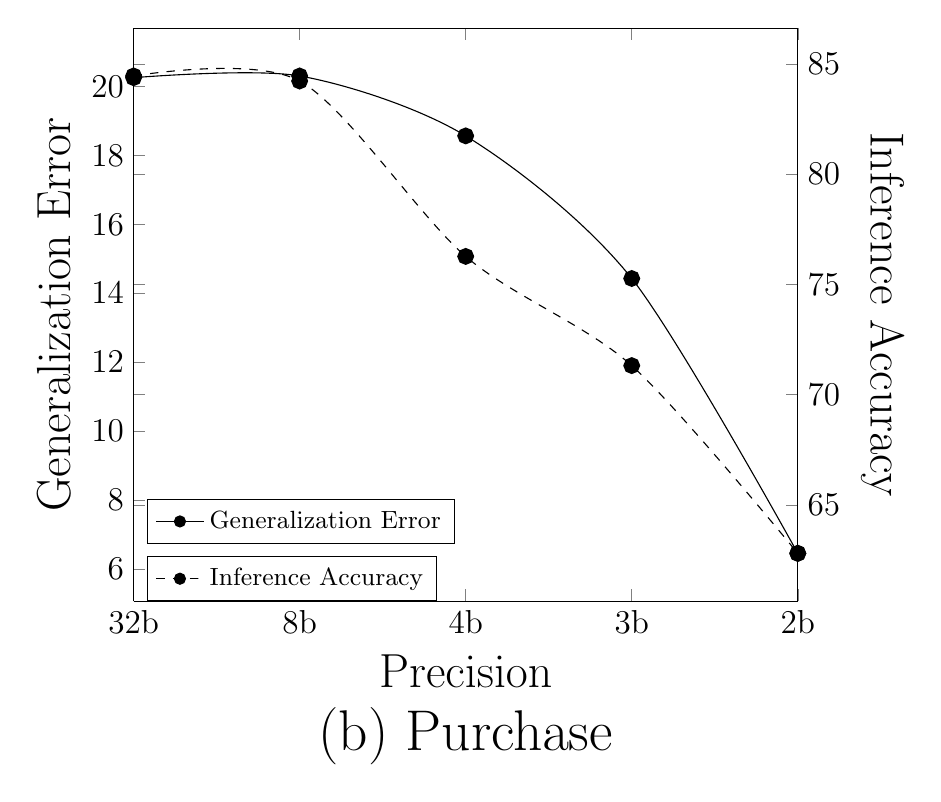
\begin{tikzpicture}
% let both axes use the same layers
\pgfplotsset{set layers}
%
\begin{axis}[
title={(b) Purchase},
title style={at={(0.5,0)},anchor=north,yshift=-40, font=\huge},
scale only axis,
line width=2.0pt,
mark size=2.0pt,
xmin=0,xmax=4,
ylabel={Generalization Error},
axis y line*=left,
xlabel={Precision},
xtick={0,1,2,3,4},
xlabel style={font=\LARGE},
ylabel style = {font=\LARGE},
xticklabel style = {font=\large},
yticklabel style = {font=\large},
xticklabels={32b, 8b, 4b, 3b, 2b},
legend style={at={(0.02,0.1)},anchor=south west, font=\small}
]
\addplot[
    color=black,
    solid,
    mark=*,
    mark options={solid},
    smooth
    ]
    coordinates {
    (0,20.26)(1,20.31)(2,18.57)(3,14.43)(4,6.45)
      };
      \addlegendimage{color=black,solid,mark=*, mark options={solid}}
      \addlegendentry{Generalization Error}
\end{axis}

\begin{axis}[
scale only axis,
line width=2.0pt,
mark size=2.0pt,
xmin=0,xmax=4,
ylabel near ticks, yticklabel pos=right,
ylabel={Inference Accuracy},
ylabel style = {rotate=180,font=\LARGE},
yticklabel style = {font=\large},
axis x line=none,
legend style={at={(0.02,0)},anchor=south west, font=\small}
]
\addplot[
    color=black,
    dashed,
    mark=*,
    mark options={solid},
    smooth
    ]
    coordinates {
    %(0,62.08)(1,62.05)(2,59.86)(3,57.27)(4,53.38)
    (0,84.45)(1,84.22)(2,76.27)(3,71.32)(4,62.81) %updated results
        };
        \addlegendimage{color=black,dashed,mark=*,mark options={solid}}
        \addlegendentry{Inference Accuracy}
\end{axis}
\end{tikzpicture} &





%
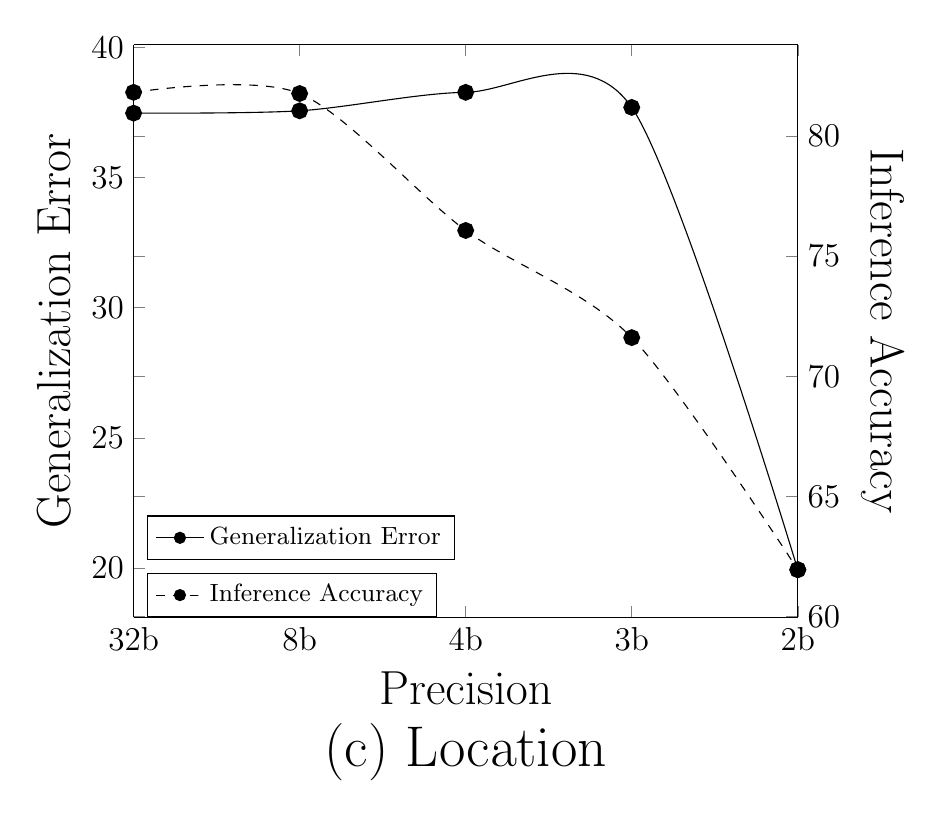
\begin{tikzpicture}
% let both axes use the same layers
\pgfplotsset{set layers}
%
\begin{axis}[
title={(c) Location},
title style={at={(0.5,0)},anchor=north,yshift=-40, font=\huge},
scale only axis,
line width=2.0pt,
mark size=2.0pt,
xmin=0,xmax=4,
ylabel={Generalization Error},
axis y line*=left,
xlabel={Precision},
xtick={0,1,2,3,4},
xlabel style={font=\LARGE},
ylabel style = {font=\LARGE},
xticklabel style = {font=\large},
yticklabel style = {font=\large},
xticklabels={32b, 8b, 4b, 3b, 2b},
legend style={at={(0.02,0.1)},anchor=south west, font=\small}
]
\addplot[
    color=black,
    solid,
    mark=*,
    mark options={solid},
    smooth
    ]
    coordinates {
    (0,37.48)(1,37.57)(2,38.28)(3,37.70)(4,19.93)
      };
      \addlegendimage{color=black,solid,mark=*, mark options={solid}}
      \addlegendentry{Generalization Error}
\end{axis}

\begin{axis}[
scale only axis,
line width=2.0pt,
mark size=2.0pt,
xmin=0,xmax=4,
ylabel near ticks, yticklabel pos=right,
ylabel={Inference Accuracy},
ylabel style = {rotate=180,font=\LARGE},
yticklabel style = {font=\large},
axis x line=none,
legend style={at={(0.02,0)},anchor=south west, font=\small}
]
\addplot[
    color=black,
    dashed,
    mark=*,
    mark options={solid},
    smooth
    ]
    coordinates {
    (0,81.82)(1,81.77)(2,76.07)(3,71.61)(4,61.95)
        };
        \addlegendimage{color=black,dashed,mark=*,mark options={solid}}
        \addlegendentry{Inference Accuracy}
\end{axis}
\end{tikzpicture}


\end{tabular}
}
\caption{Pruning followed by quantization (i.e., weight sharing) restores the predictive accuracy while limiting information leakage (i.e., generalization error).}
%\caption{\underline{Pruning followed by Weight Sharing (Quantization).} While the retraining after pruning is necessary to restore the predictive accuracy, clustering the weights to reduce the precision lowers the inference accuracy risk while reducing the generalization error for FashionMNIST(left), Purchase100(Center) and Location(Right) dataset.}
\label{fig:wtsharing}
\end{center}
\end{figure*}
